\documentclass{emulateapj}
%\documentclass[12pt,preprint]{aastex}

\usepackage{graphicx}
\usepackage{float}
\usepackage{amsmath}
\usepackage{hyperref}
\usepackage[caption=false]{subfig}
\usepackage{epsfig,floatflt}



\begin{document}

\title{A spectacular title}

\author{Daniel Heinesen}

\email{daniel.heinesen@sf-nett.no}

\altaffiltext{1}{Institute of Theoretical Astrophysics, University of
  Oslo, P.O.\ Box 1029 Blindern, N-0315 Oslo, Norway}


%\date{Received - / Accepted -}

\begin{abstract}
  State problem. Briefly describe method and data. Summarize main results.
\end{abstract}
\keywords{cosmic microwave background --- cosmology: observations --- methods: statistical}

\section{Introduction}
\label{sec:introduction}




%Discuss background, physical importance and possibly some history of
%the problem that is being studied in this paper.


\section{Method}
The method described here is a taken from \emph{REF OPPGAVETEKST}. For a more detailed description we refer you to this paper \emph{EVT SAME REF}.
\label{sec:method}

\subsection{Data Model}
CMB can be well approximated as a Gaussian distribution \emph{REF}
\begin{equation}
p(\mathbf{d}) = \frac{1}{\sqrt{|\mathbf{C}|}}e^{-\frac{1}{2}\mathbf{d}^T \mathbf{C}^{-1}\mathbf{d}}.
 \end{equation} 

Here $\mathbf{d}$ is the observed data, and $\mathbf{C}$ the covariance matrix for the pixels in the CMB field.

We are taking the observed CMB data $d(\hat{n})$ to be consisting of three parts
\begin{equation}
d(\hat{n}) = s(\hat{n}) + f(\hat{n}) + n(\hat{n}),
\end{equation}
where $f$ is the foreground radiation, $n$ is the noise and $s$ is the actual signal from the CMB. We assume that non of these are correlated, and we can therefore write the covariance matrix for the data $d$ as 
\begin{equation}
\mathbf{C} = \langle \mathbf{d}\mathbf{d}^T\rangle = \mathbf{S} + \mathbf{N} + \mathbf{F},
\end{equation}
where $\mathbf{S}$, $\mathbf{N}$ and $\mathbf{F}$ are the covariance matrices from $s$, $n$ and $f$ respectively. We so need to find expression for these matrices. 

We start with the foreground. We want to marginalize over the the dipole and monopole so to not get any contributions from these. This is done with a map of the structures we want to ignore $\mathbf{f}$ and a large number $\lambda$:
\begin{equation}
\mathbf{F} = \lambda \mathbf{f}\mathbf{f}^T.
\end{equation}

This gives these regions near infinite variance, and is thus ignored.

We do not expect the noise in the different pixels to be correlated to one another, so $N$ will be a diagonal matrix defined as
\begin{equation}
\mathbf{N} = \langle n_i n_j\rangle = \sigma_i^2\delta_{ij}.
\end{equation}

The last part of the covariance matrix is the actual CMB: $\mathbf{S}$. \emph{REF} shows that this can be written as 
\begin{equation}
S_ij = \frac{1}{4\pi}\sum_{\ell=0}(2\ell + 1)(b_\ell p_\ell)^2 C_\ell P_\ell(\cos\theta_{ij}),
\end{equation}
where $b_\ell$ is the instrumental beam, $p_\ell$ is the pixel window \emph{REF EVT THEORY}, $P_\ell$ are Legendre polynomials and $\theta_{ij}$ is the angle between two pixels $i$ and $j$. $C_\ell$ refers to the power spectrum 
\begin{equation}
C_\ell = |a_\ell|^2.
\end{equation}

We use the power law model of the power spectrum given in \emph{REF}, with $P(k) \propto k^n$. In this model it can be shown that $C_\ell$ can be given as
\begin{equation}
C_\ell = \frac{4\pi}{5}Q^2\frac{\Gamma\left(\ell + \frac{n-1}{2}\right)\Gamma\left(\frac{9-n}{2}\right)}{\Gamma\left(\ell + \frac{5-n}{2}\right)\Gamma\left(\frac{3+n}{2}\right)}.
\end{equation}

To ease the numerical calculation we write this recursively
\begin{equation}
C_{\ell + 1} = C_\ell \frac{2\ell + n -1}{2\ell + 5 - n}.
\end{equation}

Since we are not interested in the mono- and dipole we let $C_0 = C_1 = 0$, and for simplicity we let $C_2 = 4\pi/5Q^2$.

We see that this model for the power spectrum is parametrized the amplitude $Q$ and the spectral index $n$. This also make the covariance matrix\emph{REF COV MAT} and the probability \emph{REF PROB} dependent on these parameters.

\subsection{Likelihood and Markov Chain Mote Carlo Methods}
We are interested in finding the parameters $Q$ and $n$ which gives a power spectrum that represent the observed data. We are looking for the posterior probability
\begin{equation}
P(Q,n|\mathbf{d}) = \mathcal{L}(Q,n)P(Q,n),
\end{equation}
where $P(Q,n)$ is an unknown prior probability \emph{DOUBLE CHECK} and $\mathcal{L}$ is the likelihood
\begin{equation}
\mathcal{L}(Q,n) = p(\mathbf{d}|Q,n),
\end{equation}
where $p(\mathbf{d}|Q,m)$ is the conditional probability that we are going to we will observe our data $\mathbf{d}$ given the parameters $Q$ and $n$. Due to numerical limits of our numerical methods, we are not interested in $\mathcal{L}$ directly, but rather its logarithm, given as \emph{REF HANS-KRISTIAN}
\begin{equation}
-2\log \mathcal{L}(Q,n) =  \mathbf{d}^T\mathbf{C}^{-1}\mathbf{d} + \log|\mathbf{C}|.
\end{equation}

To make everything more computationally faster, we do a Cholesky decomposition of the covariance matrix:
\begin{equation}
\mathbf{C} = \mathbf{L}\mathbf{L}^T.
\end{equation} 
 
This makes the inversion easier
\begin{equation}
\mathbf{d}^T\mathbf{C}^{-1}\mathbf{d} = \mathbf{x}^T\mathbf{x} \Leftrightarrow \mathbf{x} = \mathbf{L}^{-1}\mathbf{d},
\end{equation}

since solving the triangular matrix system $\mathbf{L}\mathbf{d} = \mathbf{x}$ is faster than inverting $\mathbf{C}$. The triangular matrix $\mathbf{L}$ also gives us the advantage at
\begin{equation}
\log|\mathbf{C}| = \log |\mathbf{L}\mathbf{L}^T| = 2\sum_i \log L_{ii}.
\end{equation}

To find this distribution \emph{REF DIST} we are using a Markov Chain Monte Carlo method, namely the Metropolis-Hastings algorithm \emph{REF BOOK}\footnote{To be more precise: Since the probability distribution is symmetric the Markov chain is reversible, our proposal distribution is thus the same backwards and forward, and the algorithm reduces to a normal Metropolis algorithm.}, with the acceptance probability
\begin{equation}
P(Q_i,n_i) = \min\left(1,e^{\mathcal{L}(Q_{i},n_{i})-\mathcal{L}(Q_{i-1},n_{i-1})}\right).
\end{equation} 
But due to $\mathcal{L}(Q_{i},n_{i})-\mathcal{L}(Q_{i-1},n_{i-1})$ being able to take from very small to very large values, the exponent of this is numerically dangerous. We instead calculate this probability as
\begin{equation}
P(Q_i,n_i) = e^{p}
\label{eq:AccProb}
\end{equation}
where
\begin{equation}
p = \min\left(0,\mathcal{L}(Q_{i},n_{i})-\mathcal{L}(Q_{i-1},n_{i-1})\right)
\end{equation}
This is equivalent, but way safer numerically. With this acceptance probability we implement the algorithm


\begin{itemize}
\item Choose initial guess for $Q$ and $n$
\item loop
    \begin{itemize}
     \item move $Q$ and $n$ a step length times a uniformly random number
     \item calculate the acceptance probability \eqref{eq:AccProb}
     \item draw a uniformly distributed number $\mathbf{x}$
     \item if $\mathbf{x} < P(Q_i,n_i)$
     \begin{itemize}
     \item save $Q_i$ and $n_i$
     \end{itemize}
     \item else
     \begin{itemize}
     \item save the previous $Q_{i-1}$ and $n_{i-1}$ again
     \end{itemize}
     \end{itemize}
\end{itemize}

This algorithm will randomly walk through the posterior probability, landing more often on the more likely $Q$'s and $n$'s, and will therefore quickly converge towards the most likely $Q$ and $n$.




%
%Describe method. Define data model and likelihood. Outline how the
%likelihood was computed (grid or MCMC).
%
%Define the power law model in terms of $Q$ and $n$. 

\section{Data}
\label{sec:data}

In this article data from the COBE satellite is used. We look at $53$ and $90$ GHZ map, since they gives the cleanest data. For the collection of the data a $7^{\circ}$ beam was used. The foreground was masked out, so not to contaminate the data with noise from stars and galactic dust. $\ell$ was used in an interval of $0$ to $47$. 


%Summarize properties of data. Which data are used (experiment,
%frequencies etc.)? Pixel resolution ($N_{\textrm{side}}$),
%$\ell_{\textrm{max}}$ -- everything necessary to repeat the analysis
%for other researchers.
%
%Show a sky map of the smoothed data. Use the Healpix routine
%``smoothing'' to do this; it works just like anafast. Smooth with a
%$7^{\circ}$ beam, and plot with ``map2gif''. Show the RMS pattern as
%well. 

\section{Results}
\label{sec:results}

\begin{figure}[t]
\centering
\subfloat[Posterior distribution for $53$ GHz]{
\includegraphics[scale=0.4]{mcmc53Dist.png}
}\\
\subfloat[Posterior distribution for $90$ GHz]{
\includegraphics[scale=0.4]{mcmc90Dist.png}
}
\caption{Posterior distribution for the amplitude $Q$ and the tilt $n$, found with $2\cdot 10^4$ Metropolis iteration, and the contour plots made with a resolution of $250$. Due to the relatively low number of iteration, the data is quite sparse and the contour plot fragmented. }
\end{figure}

\begin{table}[t]
\centering
\begin{tabular}{c | c | c}
& $53$ GHz & $90$ GHz \\
\hline
$n$ & $0.696 \pm 0.381$ & $0.915 \pm 0.623$\\
$Q[\mu K]$ & $16.3 \pm 3.81$ & $18.9 \pm 6.12$
\end{tabular}
\caption{Results for the Monte Carlo simulation with $2\cdot 10^4$ Metropolis iteration. The results are on the form $\mu \pm \sigma$ and are taken directly from the values we get from the random walk, and is not calculated from the distribution in fig. \ref{fig:QnDist}}
\label{tab:results}
\end{table}

\begin{figure}[t]
\centering
\subfloat[Posterior distribution $P(Q|\mathbf{d})$]{
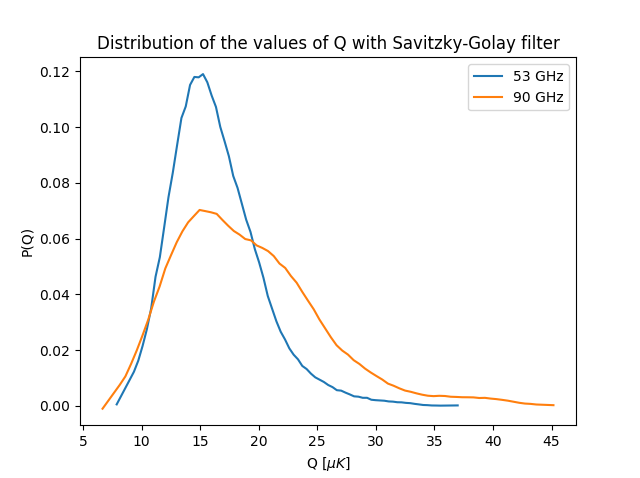
\includegraphics[scale=0.4]{mcmcJointQSavgol.png}
}\\
\subfloat[Posterior distribution $P(n|\mathbf{d})$]{
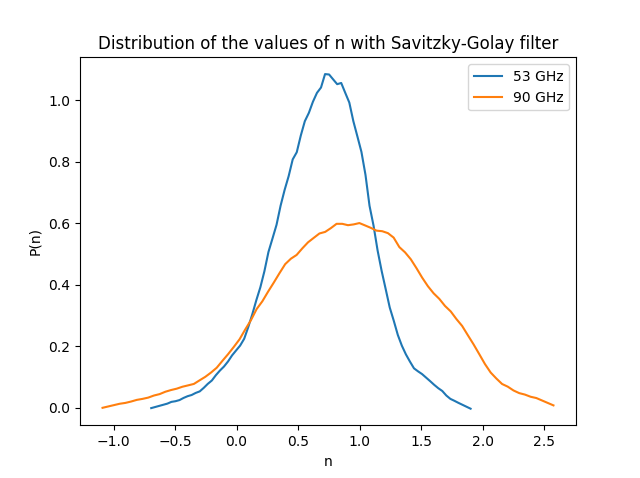
\includegraphics[scale=0.4]{mcmcJointnSavgol.png}
}
\caption{Posterior distribution $P(n|\mathbf{d})$ and $P(Q|\mathbf{d})$ with $2\cdot 10^4$ Metropolis iteration and a resolution of $250$. Due to the few Metropolis iterations, the raw results are quite messy, so a Savitzky-Golay filter is used to smooth the data with out loss of generality \emph{SKJEKK DETTE!!!!}}
\label{fig:QnDist}
\end{figure}


The Monte Carlo simulations run with $2\cdot 10^4$ Metropolis iterations and take around about $80$ minutes. The result of simulation for $53$ and $90$ GHz are summarized in table \ref{tab:results}.\

The 







%Show the 2D likelihood contours. Summarize constraints on $Q$ and
%$n$. 


\section{Conclusions}
\label{sec:conclusions}

Summarize results. Discuss their importance, referring to the
discovery to the initial seeds for structure formation. Mention that
these results are in good agreement with expectations from
inflationary theory.





%\begin{deluxetable}{lccc}
%%\tablewidth{0pt}
%\tablecaption{\label{tab:results}}
%\tablecomments{Summary of main results.}
%\tablecolumns{4}
%\tablehead{Column 1  & Column 2 & Column 3 & Column 4}
%\startdata
%Item 1 & Item 2 & Item 3 & Item 4
%\enddata
%\end{deluxetable}



\begin{acknowledgements}
  Who do you want to thank for helping out with this project?
\end{acknowledgements}

\begin{thebibliography}{}

\bibitem[G{\'o}rski et al.(1994)]{gorski:1994} G{\'o}rski, K. M.,
  Hinshaw, G., Banday, A. J., Bennett, C. L., Wright, E. L., Kogut,
  A., Smoot, G. F., and Lubin, P.\ 1994, ApJL, 430, 89

\end{thebibliography}


\end{document}
